\documentclass[red]{beamer}
\usetheme{CambridgeUS}
\setbeamertemplate{navigation symbols}{}
\setbeamertemplate{footline}{}
\setbeamertemplate{items}[triangle] 
\renewcommand{\footnoterule}{}

\usepackage[utf8]{inputenc}
\usepackage[slovak]{babel}
\usepackage[IL2]{fontenc}
\usepackage[protrusion=true,expansion=true]{microtype}
\usepackage[none]{hyphenat}

\usepackage{hyperref}
\urlstyle{same}
\usepackage{textcomp}
\usepackage{xargs}
\usepackage{graphicx}
\usepackage{wrapfig}
\usepackage[absolute,overlay]{textpos}
\usepackage{amssymb}
\usepackage{amsmath}
\usepackage{verbatim}
\usepackage{eurosym}

\newcommand{\TODO}{{\color{red}!!!!!!!!!!!!!!!!!!!!!!!!}}
\newcommand{\vlnovka}{\raise.35ex\hbox{$\scriptstyle\mathtt{\sim}$}}

\newcommandx{\odrazka}[3][1=1, 2]{\begin{itemize}\item<#1-#2> #3\end{itemize}}



%%%%%%%%%%%%%%%%%%%%%%%%%%%%%%%%%%%%%%%%%%%%%%%%%%

\begin{document}

\large

\title{Odstraňovanie tieňov}
\subtitle{Spracovanie farebného obrazu}
\author{Rastislav Kamenický, Michal Piovarči, Matej Kopernický}
\date{14.5.2013}

{
\setbeamertemplate{background canvas}{
\includegraphics[width=\paperwidth,height=\paperheight]{title}}
\begin{frame}[plain,t]
\begin{center}
\color{white}
\vspace{2,5cm}
\huge\inserttitle\\
\vspace{0.9cm}
\Large\insertsubtitle\\
\vspace{1.75cm}
\color{black}
\large\insertauthor\\
\bigskip\bigskip
\href{http://www.github.com/misop/shadow_removal}{github.com/misop/shadow\_removal}
\end{center}
\end{frame}
}



\begin{frame}
\begin{columns}
\begin{column}{0.59\textwidth}
\odrazka[1]{Široké využitie pri úprave fotografií}
\odrazka[2]{Neexistuje žiadne 100\% riešenie}
\odrazka[3]{Väčšinou sú vyžadované parametre snímacieho zariadenia, vlastnosti scény a pod.}
\odrazka[4]{Cieľ -- vytvoriť jednoduchú metódu, ktorej vstupom je len obrázok a je potrebné len minimum interakcie}
\end{column}
\begin{column}{0.4\textwidth}
\uncover<1->{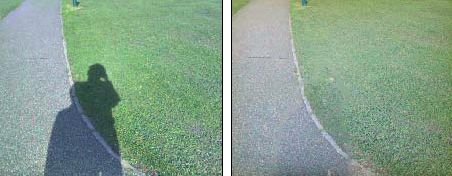
\includegraphics[width=\linewidth]{./img/1.jpg}}\\
\bigskip
\uncover<1->{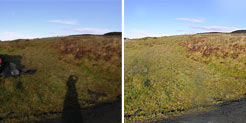
\includegraphics[width=\linewidth]{./img/2.jpg}}
\end{column}
\end{columns}
\end{frame}



\begin{frame}
\odrazka{Hlavné zdroje:}
G. D. Finlayson, M. S. Drew, C. Lu: \textit{Intrinsic Images by Entropy Minimization}, European Conference on Computer Vision, Vol. 3 (2004), pp. 582-595\\
\medskip
G. D. Finlayson, M. S. Drew, C. Lu: \textit{Entropy Minimization for Shadow Removal}, Int. J. Comput. Vision, Vol. 85 (2009), pp. 35--57\\
\bigskip
\pause
\odrazka{Intrinsic image: obrázok nezávislý od svetla, a teda aj zbavený tieňov}
\pause
\odrazka{Entropia: \uv{neusporiadanosť, zložitosť} obrázku}
\end{frame}



\begin{frame}{Postup}
\begin{itemize}[<+->]
\item Nájsť intrinsic obrázok
\item Na základe neho identifikovať tieň
\item Odstrániť tieň
\end{itemize}
\end{frame}


\begin{frame}{Chromaticity}
\odrazka{Špecifikácia farby nezávisle na osvetlení}
\pause
\odrazka{Chromaticity colour space
\begin{enumerate}
\item greyscale 1D invariant chromaticity\\
$\{log(G/R), log(B/R)\}$
\item 2D invariant L1 chromaticity\\
$X = [\log(R/\sqrt[3]{R*G*B}), \log(G/\sqrt[3]{R*G*B}), \log(B/\sqrt[3]{R*G*B})]$\\
$\{ [\frac{1}{\sqrt{2}}, -\frac{1}{\sqrt{2}}, 0] * X^T,  [\frac{1}{\sqrt{6}}, -\frac{1}{\sqrt{6}}, -\frac{2}{\sqrt{6}}] * X^T \}$
\end{enumerate}
}
\end{frame}



\begin{frame}{Chromaticity}
\odrazka[1]{Zmena v osvetlení v praxi zodpovedá posunu v chromatickom priestore jedným smerom (za predpokladu jedného zdroju svetla)}
\odrazka[2]{Hľadáme orientáciu pixelov v chromatickom priestore}
\vspace{-.1cm}
\uncover<1->{\centerline{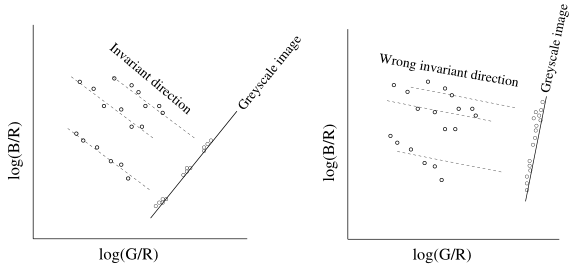
\includegraphics[width=.75\linewidth]{./img/chromaticity_example}}}
\end{frame}



\begin{frame}{Hľadanie orientácie}
\odrazka{Projekciou bodov na priamku vo vhodnom smere $\theta$ získame šedoúrovňový obrázok}
$$ \mathcal{I} = \chi_1 cos\theta + \chi_2 sin\theta $$
\pause
\odrazka{Najvhodnejší smer $\theta$ nájdeme mnimalizáciou entropie}
$$ -\sum_i p(x_i)*\log p(x_i) $$
\end{frame}



\begin{frame}{Výpočet entropie}
\odrazka{Nepresnosti v reálnych fotkách -- vstupný obrázok vyhladíme Gaussianom}
\pause
\odrazka{Vytoríme histogram šedoúrovňového obrázku, vezmeme iba 90\% stredných dát}
\pause
\odrazka{\uv{Bin width} histogramu na základe Scottovho pravidla}
$$ 3.5 std(data)\sqrt[3]{N} $$
\pause
\odrazka{po normalizácii histogramu a vylúčení malých hodnôt získame entropiu}
$$ \eta = - \sum_i p_i \log p_i $$
\vspace{-.3cm}
\centerline{$p_i$ -- veľkosť \uv{binov} histogramu}
\end{frame}



%rovnaka velkost pisma pre subitemize
\setbeamerfont*{itemize/enumerate subbody}{parent=itemize/enumerate body}

\begin{frame}{Získanie intrinsic obrázku -- výsledný algoritmus}
\begin{itemize}[<+->]
\item Získaj 2D logaritmický chromatický obrázok
\item for $\theta=1..180$
\begin{itemize}[<+->]
\item Získaj šedoúrovňový obrázok $\mathcal{I}$ na základe projekcie bodov pod uhlom $\theta$
\item Vypočítaj entropiu $\mathcal{I}$
\item Ak je entropia nižšia ako doterajšie minimum, $\theta$ je najlepší odhad
\end{itemize}
\item Na základe najlepšej $\theta$ zrekonštruujeme šedoúrovňový intrinsic obrázok, pridáme energiu tak, aby medián 1\% najjasnejších pixelov mal chromaticitu pôvodného obrázku
\end{itemize}
\end{frame}



\begin{frame}
\centerline{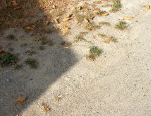
\includegraphics[width=.75\linewidth]{./img/example}}
\end{frame}

\begin{frame}
\centerline{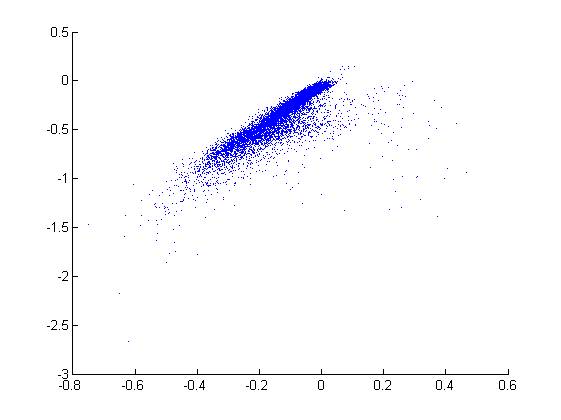
\includegraphics[width=.9\linewidth]{./img/chromaticity1}}
\end{frame}

\begin{frame}
\centerline{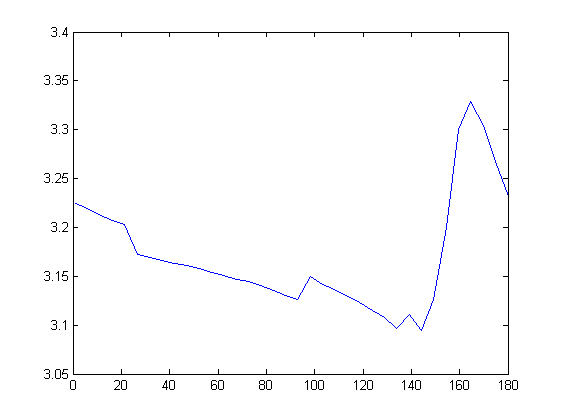
\includegraphics[width=.9\linewidth]{./img/chromaticity1_theta}}
\end{frame}

\begin{frame}
\centerline{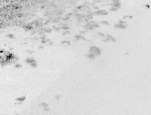
\includegraphics[width=.75\linewidth]{./img/intrinsic}}
\end{frame}



\begin{frame}{Identifikácia tieňa}
\odrazka{Ako získať tieň?}
\pause
\odrazka{Intrinsic $-$ X * šedoúrovňový obrázok}
\pause
\odrazka{Vyhladenie masky, odstránenie šumu a dier pomocou morfológie}
\pause
\bigskip
\begin{columns}
\begin{column}{.49\linewidth}
\centerline{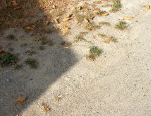
\includegraphics[width=\linewidth]{./img/example}}
\end{column}
\begin{column}{.49\linewidth}
\centerline{
\includegraphics[width=\linewidth]{./img/mask}}
\end{column}
\end{columns}
\end{frame}



\begin{frame}{Odstránenie tieňa}
\odrazka{Zvolený iný postup ako v pôvodnej práci}
\bigskip
\centerline{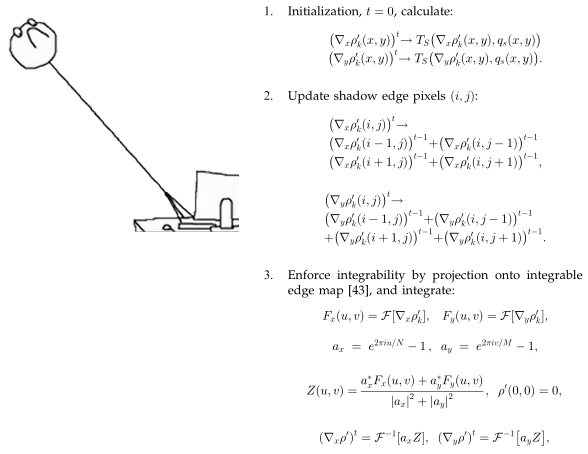
\includegraphics[width=.75\linewidth]{./img/removal_wtf}}
\end{frame}



\begin{frame}{Odstránenie tieňa  (zjednodušená verzia)}
\odrazka[1]{Nájdeme obrysy tieňa a dotyčnice k nemu}
\odrazka[2]{Na základe dotyčníc nájdeme pixely z oboch strán obrysov}
\odrazka[3]{Časť obrazu v tieni prenásobime pomerom priemernej svetlosti pixelov vo svetle a tieni}
\bigskip
\uncover<2->{\centerline{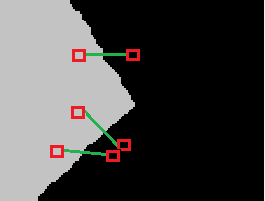
\includegraphics[width=.5\linewidth]{./img/dotycnice}}}
\end{frame}



\begin{frame}{Odstránenie tieňa}
\centerline{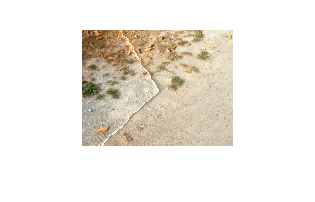
\includegraphics[width=\linewidth]{./img/result1}}
\end{frame}



\begin{frame}{Odstránenie tieňa}
\odrazka[1]{Problém pri nehomogénnom povrchu}
\odrazka[2]{Škaredé okraje}
\odrazka[3]{Pokus o ich vyhladenie vyprodukoval ešte škaredšie okraje}
\uncover<1->{\centerline{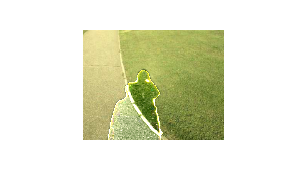
\includegraphics[width=.75\linewidth]{./img/result2}}}
\end{frame}



\begin{frame}{Odstránenie tieňa}
\odrazka{Pokus o zložitejší prístup pomocou watershed segmentácie}
\pause
\odrazka{Postupne zosvetliť oblasti v tieni od najsvetlejších okrajov smerom dovnútra}
\pause
\odrazka{Horšie výsledky než predošlá metóda}
\bigskip
\centerline{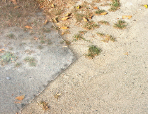
\includegraphics[width=.5\linewidth]{./img/result1_watershed}}
\end{frame}



\begin{frame}
\vspace{1cm}
\centerline{\huge\textbf{Ukážka \& Otázky}}
\vspace{2cm}
\centerline{
\includegraphics[scale=.5]{./img/zaver}}
\end{frame}



\end{document}